\section{How important is the treatment of resources from housing in determining who is poor?}\label{sec:housing}

Previous sections have shown that conclusions about the rate of growth in household resources, and the evolution of inequality and poverty, are sensitive, for most sub-periods, to the way that resources are measured. Section \ref{sec:trends} showed that adding the imputed resources from housing to our measure of household resources increases the impression of by how much living standards have grown over the past 30 years, and reduces measures of inequality. This section explores how adding the imputed resources from housing changes our impression of which households are in poverty, in a similar way to how Section \ref{sec:compositionwith} explored how income and consumption identified different groups of households as being in poverty. [And does something else too?]

\begin{figure}
\caption{Risk of Poverty, by Age and Cohort }
\centering
\begin{tabular}{c c}
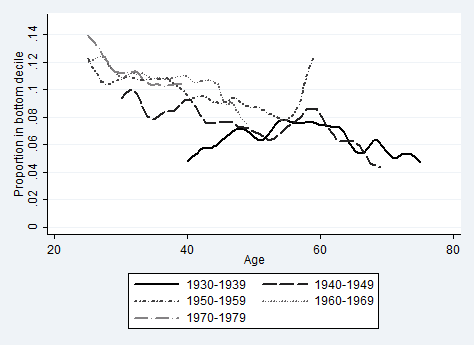
\includegraphics[width=.5\linewidth]{pictures/cohortagerisksmooth_bhc_inc.png} &
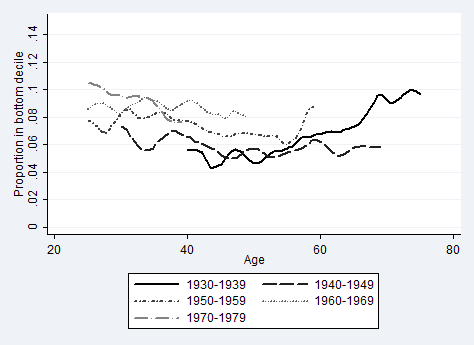
\includegraphics[width=.5\linewidth]{pictures/cohortagerisksmooth_bhc_con.png} \\
(a) Income inc. Housing & (b) Consumption inc. Housing \\
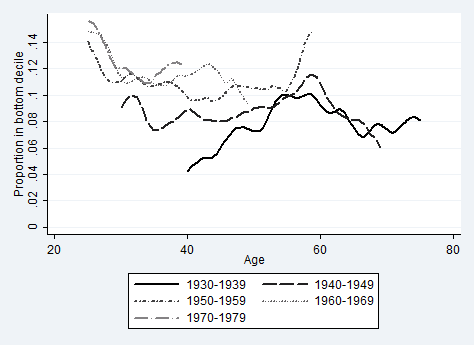
\includegraphics[width=.5\linewidth]{pictures/cohortagerisksmooth_ahc_inc.png} &
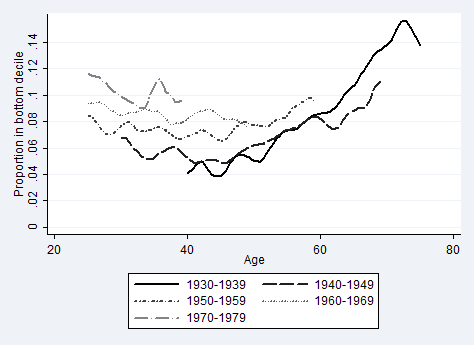
\includegraphics[width=.5\linewidth]{pictures/cohortagerisksmooth_ahc_con.png} \\
(c) Income ex. Housing & (d) Consumption ex. Housing \\
\end{tabular}
\label{fig:povage_cohort}
\end{figure}

\begin{figure}
\caption{Risk of Poverty, by Age and Cohort }
\centering
\begin{tabular}{c c}
Income & Consumption\\
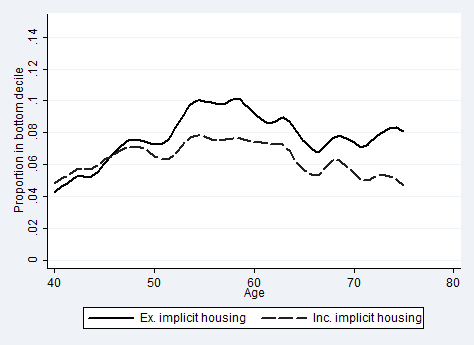
\includegraphics[width=.5\linewidth]{pictures/cohort2_agerisksmooth_inc.png} &
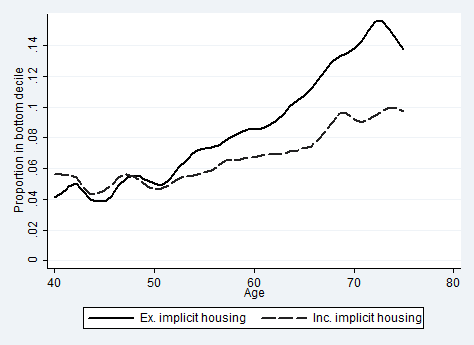
\includegraphics[width=.5\linewidth]{pictures/cohort2_agerisksmooth_con.png} \\
(a) 1930s Cohort & (b) 1930s Cohort \\
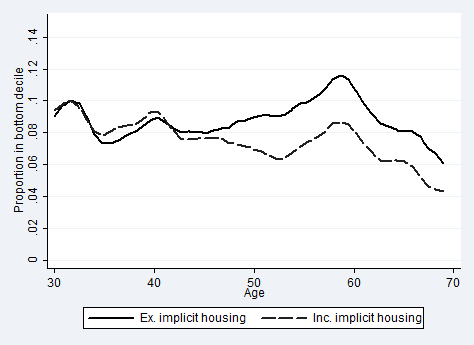
\includegraphics[width=.5\linewidth]{pictures/cohort3_agerisksmooth_inc.png} &
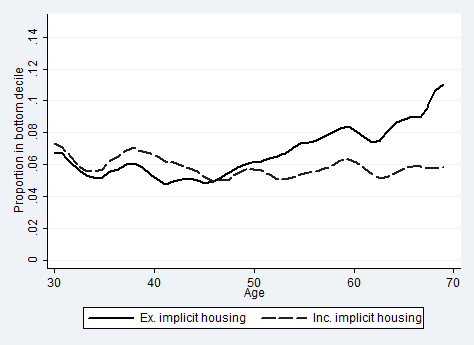
\includegraphics[width=.5\linewidth]{pictures/cohort3_agerisksmooth_con.png} \\
(c) 1940s Cohort & (d) 1940s Cohort \\
\end{tabular}
\label{fig:povage_cohort_restrict}
\end{figure}

\begin{sidewaystable}
\caption{Demographics and the Bottom Decile of IHC \& XHC Distributions, 1999-2009: Relative Risk Ratios}
\centering
\begin{tabular}{l|cccc|cccc}
\hline\hline 
	& \multicolumn{4}{c}{\textbf{Income Bottom Decile}} &  \multicolumn{4}{c}{\textbf{Cons. Bottom Decile}} \\
	&	$r_{IX}$	&	$r_{I}$	&	$r_{X}$ &	$r_{I}$-$r_{X}$&	$r_{IX}$	&	$r_{I}$	&	$r_{X}$	&	$r_{I}$-$r_{X}$\\
  & se & se & se  & $\chi^{2}$ & se & se & se & $\chi^{2}$ \\
\hline
Left school $\leq$ 16	&	       1.37***  	&	       2.51***	&	      1.45***	&	1.06****	&	     					  3.17***	&	       2.89***	&	2.79***	&	0.11	\\
                   		 	&	       0.10  	&	0.31	&	0.09	&	18	&	      
						 0.23   	&	0.33	&	0.27	&	0.08	\\
16 $<$ Left school $<=$ 19	&	       0.96   	&	       0.97  	&	1.46***	&	-0.48***	&	
				       1.08   	&	       1.01  	&	       1.78***  	&	-0.78***	\\
                    		&	       0.08   	&	0.09	&	0.14	&	7.8	&	     
					  0.08   	&	0.09	&	0.18	&	24	\\
Age $<$ 30	&	       1.92*** 	&	       1.89***  	&	1.95***	&	-0.06	&	
			       2.07***  	&	1.30***	&	1.84***	&	-0.54***	\\
                    	&	       0.13   	&	0.10	&	0.23	&	0.04	&	  
			     0.17   	&	0.10	&	0.18	&	17	\\
Age 30-40	&	      1.20***   	&	       1.44***	&	       0.99 	&	0.45***	&	
			       1.34***   	&	       1.26***	&	1.08	&	0.18***	\\
                    	&	       0.05   	&	0.10	&	0.09	&	9.5	&	  
			     0.07   	&	0.06	&	0.06	&	3.7	\\
Age 50-60	&	       0.63***	&	       0.36***	&	0.84***	&	-0.48***	&
			       0.56***	&	       0.43***	&	       0.96 	&	-0.54***	\\
                    	&	       0.02   	&	0.07	&	0.05	&	15	&	
			       0.03   	&	0.03	&	0.09	&	54	\\
Age 60-70	&	       0.16***	&	       0.17***	&	       0.27***	&	-0.10***	&	       								0.22***	&	       0.23***	&	0.53	&	-0.31***	\\
                    	&	       0.01   	&	0.02	&	0.02	&	8.4	&	
			       0.02   	&	0.02	&	0.04	&	97	\\
Age $\geq$ 70	&	       0.09***	&	       0.15***	&	       0.25***	&	-0.10***	&	    					   		0.51***	&	       0.30***	&	       1.15 	&	-0.85***	\\
                    	&	       0.01   	&	0.02	&	0.03	&	7.5	&	    
				   0.05  	&	0.03	&	0.12	&	225	\\
Workless	&	       14.7***	&	       11.7***	&	       16.1***	&	-4.47***	&	       					11.9***	&	      5.20***	&	       8.04***	&	-2.85***	\\
	&	       0.81   	&	0.91	&	1.05	&	8.1	&	
		       0.67   	&	0.50	&	0.28	&	31	\\
Self Employed	&	       3.74***	&	      1.84***	&	       2.82***	&	-0.98**	&	       							0.80***	&	       0.97&	       0.73***	&	-0.24***	\\
	&	       0.34   	&	0.22	&	0.25	&	5.5	&	
		       0.07   	&	0.09	&	0.08	&	7.3	\\
Constant            	&	       0.027**	&	       0.006***	&	0.010	&		&	
				       0.012***	&	       0.010***	&	       0.008***	&		\\
                    	&	       0.002   	&	0.001	&	       0.001 	&		&	 
			      0.001   	&	0.001	&	0.001	&		\\
\hline\hline
\multicolumn{9}{l}{Significantly different from zero at the 10\% ($\star$),  5\% ($\star\star$) and 1\% level ($\star\star\star$).} \\
\multicolumn{9}{l}{Omitted variables: Left school over 19 years old, household head aged between 40 and 50 years, employed. } 
\end{tabular}
\label{table:ahc_bhc}
\end{sidewaystable}

\begin{sidewaystable}
\caption{Demographics and the Bottom Decile of IHC \& XHC Distributions, 1999-2009: Relative Risk Ratios}
\centering
\begin{tabular}{l|cccc|cccc}
\hline\hline 
	& \multicolumn{4}{c}{\textbf{Income Bottom Decile}} &  \multicolumn{4}{c}{\textbf{Cons. Bottom Decile}} \\
	&	$r_{IX}$	&	$r_{I}$	&	$r_{X}$ &	$r_{I}$-$r_{X}$&	$r_{IX}$	&	$r_{I}$	&	$r_{X}$	&	$r_{I}$-$r_{X}$\\
  & se & se & se  & $\chi^{2}$ & se & se & se & $\chi^{2}$ \\
\hline
Left school $\leq$ 16	&	       1.34***  	&	       2.09***	&	      1.49***	&	0.60**	&	     					  2.70***	&	       2.54***	&	2.85***	&	-0.32	\\
                   		 	&	       0.10  	&	0.26	&	0.11	&	6.0	&	      
						 0.23   	&	0.28	&	0.30	&	0.64	\\
16 $<$ Left school $<=$ 19	&	       1.00   	&	       0.85*  	&	1.71***	&	-0.58***	&	
				       0.83   	&	       0.92  	&	       1.78***  	&	-0.79***	\\
                    		&	       0.08   	&	0.08	&	0.14	&	12	&	     
					  0.06   	&	0.08	&	0.17	&	31	\\
Age $<$ 30	&	       1.79*** 	&	       1.95***  	&	1.61***	&	0.34	&	
			       1.83***  	&	1.57***	&	1.51***	&	0.07	\\
                    	&	       0.13   	&	0.19	&	0.18	&	1.4	&	  
			     0.178  	&	0.15	&	0.15	&	0.23	\\
Age 30-40	&	      1.14***   	&	       1.31***	&	       0.91	&	0.40***	&	
			       1.21***   	&	       1.28***	&	1.01	&	0.27***	\\
                    	&	       0.05   	&	0.10	&	0.09	&	8.2	&	  
			     0.06 	&	0.06	&	0.07	&	9.4	\\
Age 50-60	&	       0.71***	&	       0.73	&	0.81***	&	-0.08	&
			       0.78***	&	       0.74***	&	       0.95 	&	-0.21**	\\
                    	&	       0.03   	&	0.16	&	0.07	&	0.1	&	
			       0.05   	&	0.05	&	0.09	&	4.9	\\
Age 60-70	&	       0.19***	&	       0.57***	&	       0.23***	&	0.34***	&	       								0.37***	&	       0.60***	&	0.50***	& 0.10**	\\
                    	&	       0.02   	&	0.07	&	0.02	&	19	&	
			       0.03   	&	0.04	&	0.09	&	4.7	\\
Age $\geq$ 70	&	       0.10***	&	       0.54***	&	       0.17***	&	0.37***	&	    					   		0.79**	&	       0.86***	&	      0.90 	&	-0.04	\\
                    	&	       0.01   	&	0.06	&	0.02	&	30	&	    
				   0.08  	&	0.07	&	0.12	&	0.47	\\
Workless	&	       12.5***	&	       10.3***	&	       11.9***	&	-1.64	&	       									9.42***	&	      5.16***	&	       5.35***	&	-0.20***	\\
	&	       0.69   	&	0.89	&	0.73	&	1.4	&	
		       0.51   	&	0.50	&	0.19	&	0.15	\\
Self Employed	&	       3.88***	&	      1.69***	&	       3.41***	&	-1.72***	&	       							0.81**	&	       0.90 &	       0.89	&	0.01	\\
	&	       0.35   	&	0.21	&	0.31	&	14	&	
		       0.07   	&	0.09	&	0.09	&	0.03	\\
Couple	&	       0.87	&	      0.68***	&	       1.53***	&	-0.84***	&	       							0.68***	&	       0.58*** &	       1.09	&	-0.52***	\\
	&	       0.07  	&	0.08	&	0.16	&	40	&	
		       0.05   	&	0.05	&	0.17	&	14	\\
Single	&	       1.66***	&	      0.92	&	       6.46***	&	-5.55***	&	       							1.59***	&	       0.60***&	      6.66*** &	-6.05***	\\
	&	       0.14   	&	0.12	&	0.71	&	297	&	
		       0.13   	&	0.04	&	1.04	&	239	\\
Child Dummy	&	       1.27***	&	      5.36***	&	      0.72***	&	4.64***	&	       							2.09***	&	       3.80*** &	       0.77***	&	3.04***	\\
	&	       0.09   	&	0.59	&	0.06	&	289	&	
		       0.10   	&	0.22	&	0.06	&	378	\\
Constant            	&	       0.023**	&	       0.003***	&	0.004***	&		&	
				       0.010***	&	       0.006***	&	       0.004***	&		\\
                    	&	       0.002   	&	0.001	&	       0.001 	&		&	 
			      0.001   	&	0.001	&	0.001	&		\\
\hline\hline
\multicolumn{9}{l}{Significantly different from zero at the 5\% ($\star\star$) and 1\% level ($\star\star\star$).} \\
\multicolumn{9}{l}{Omitted variables: Left school over 19 years old, household head aged between 40 and 50 years, employed. } 
\end{tabular}
\label{table:ahc_bhc}
\end{sidewaystable}



\begin{figure}
\caption{Average Rooms Occupied per Person}
\centering
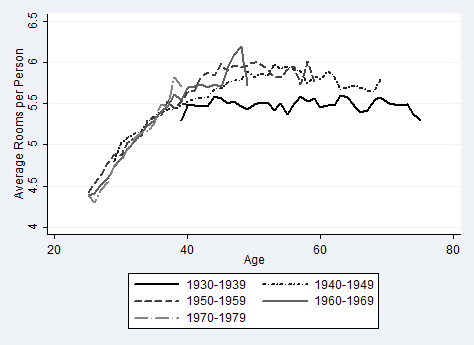
\includegraphics[width=.7\linewidth]{pictures/cohort_rooms.png}
\label{fig:cohort_rooms}
\end{figure}

\begin{figure}
\caption{Average People in Household}
\centering
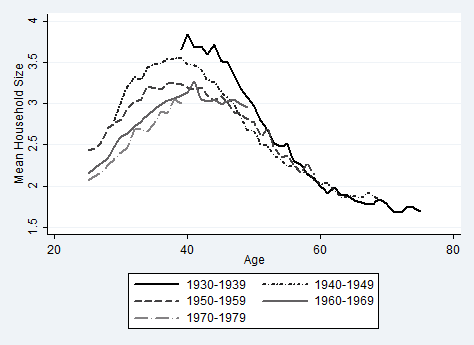
\includegraphics[width=.7\linewidth]{pictures/av_peep.png}
\label{fig:cohort_peeps}
\end{figure}


